\documentclass[12pt]{report} 
\usepackage{import}
\import{utils/}{utils.TeX}
\import{utils/}{math.TeX}
\import{utils/}{env.TeX}
\usepackage{pdfpages}
\usepackage{subfiles}


\addglobalbib{./ref.bib}
% \renewcommand*{\bibfont}{\small}

\externaldocument{./chapters/5-tnp/tnp}
\externaldocument{./chapters/6-1d/1d}
\externaldocument{./chapters/7-2d/2d}
\externaldocument{./chapters/10-appendix/model}

\newcommand{\lrtitle}{
	Unifying Transformers and Convolutional Neural Processes
}
\newcommand{\displaydate}{
	May 2024
}

\begin{document}

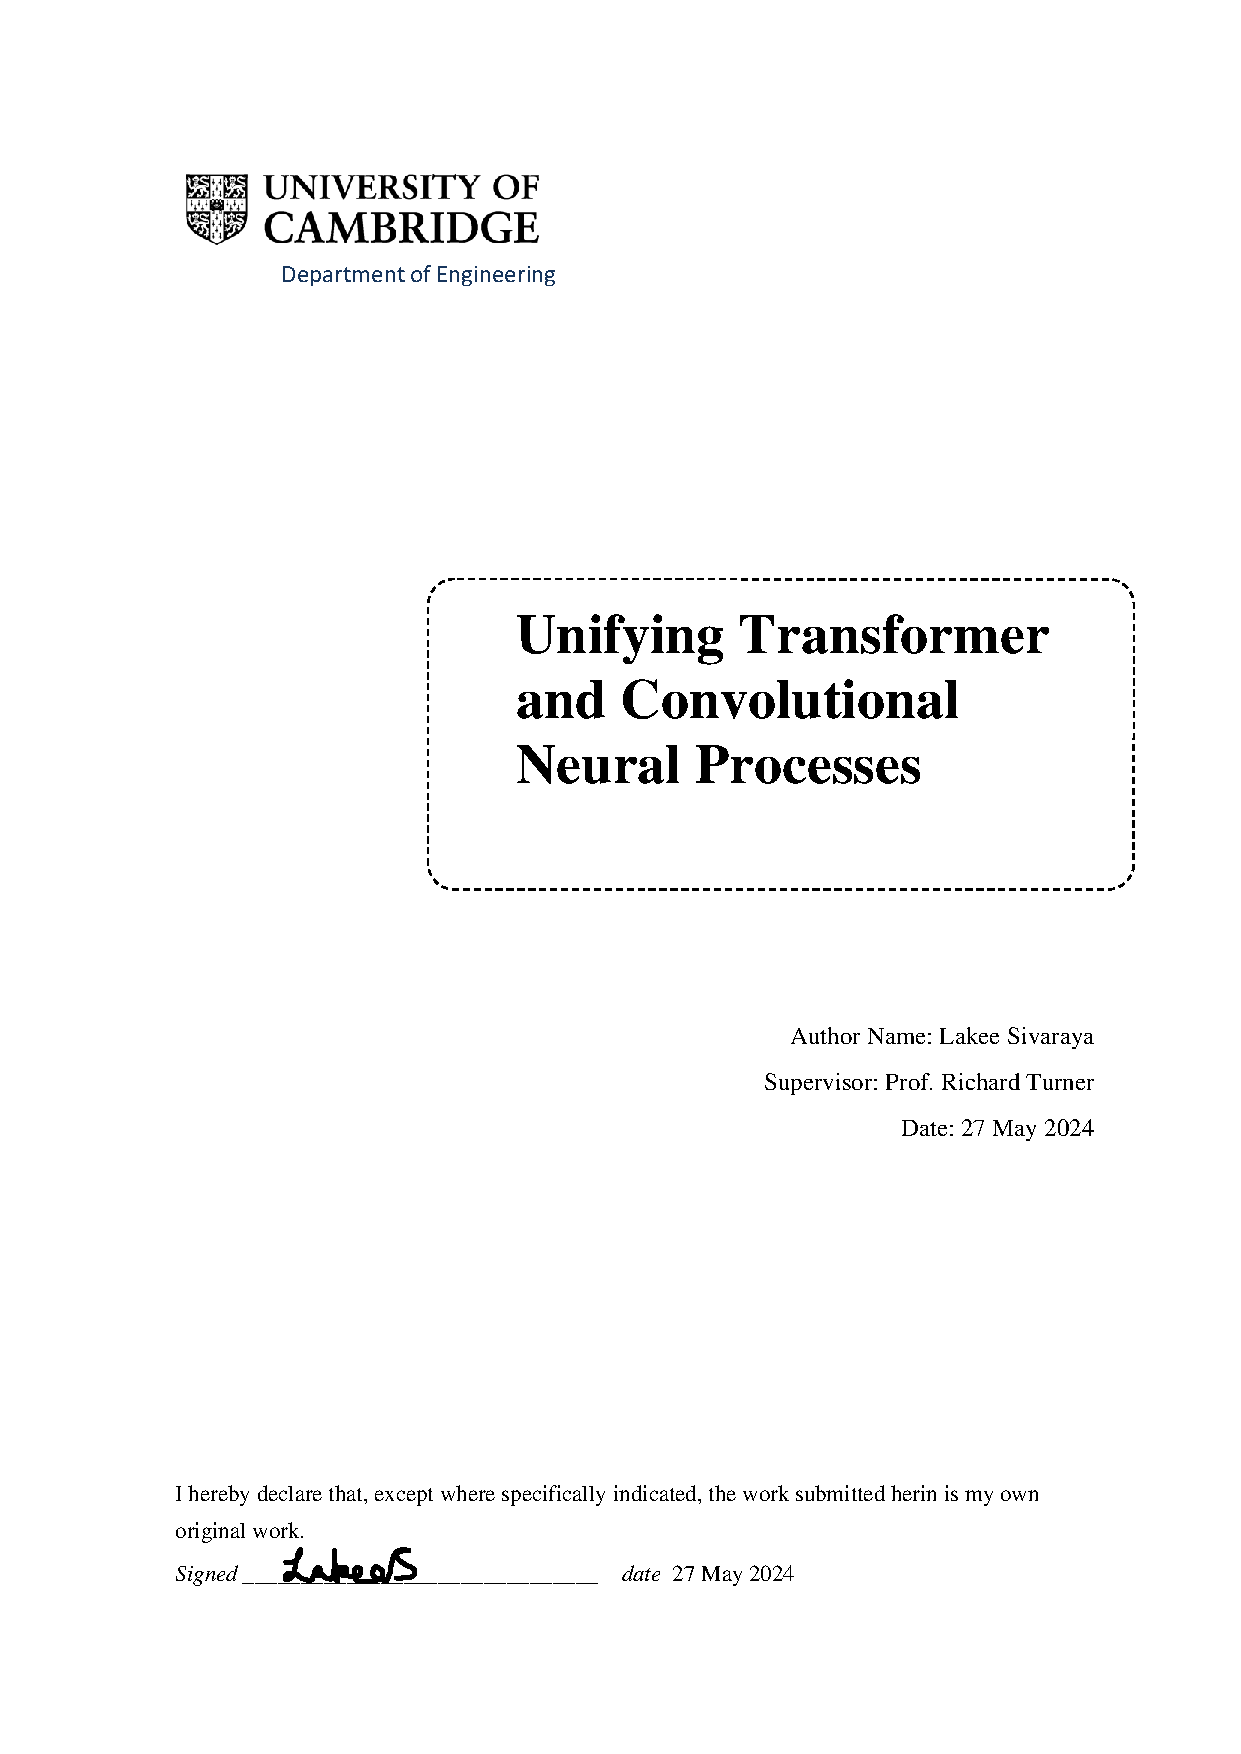
\includepdf[pages=-]{chapters/_misc/cover.pdf}

\title{\textbf{\fontsize{24.88}{12}\selectfont \lrtitle}}
\author{{\LARGE \name}}

\reporttitlepage

\chapter*{Acknowledgement}
\subfile{chapters/_misc/acknowlegement.tex}
\newpage
\chapter*{Abstract}
\subfile{chapters/0-abstract/abstract.tex}

\TOC{gray}


\chapter{Introduction}
\subfile{chapters/1-introduction/index.tex}

\chapter{Neural Processes}
\subfile{chapters/2-neural-process/neural-process.tex}

\chapter{Convolutional Neural Processes}
\subfile{chapters/3-convcnp/convcnp.tex}

\chapter{Transformer Neural Processes}
\subfile{chapters/4-transformer/transformer.tex}
\subfile{chapters/5-tnp/tnp.tex}

\chapter{Experimentation on 1D Datasets}
\subfile{chapters/6-1d/1d.tex}

\chapter{Experimentation on 2D Datasets}
\subfile{chapters/7-2d/2d.tex}

\chapter{Linear Runtime Models}
\subfile{chapters/8-linear-transformer/linear-transformer.tex}

\chapter{Conclusion}
\subfile{chapters/9-conclusion/conclusion.tex}


\printbibliography[heading=bibintoc]{}



\newpage
 

\begin{appendices}
\chapter{Model Configuration}
\subfile{chapters/10-appendix/model.tex}
\chapter{Risk Assessment}
\subfile{chapters/10-appendix/risk.tex}

\end{appendices}



\end{document}